Django es parte de una ola de frameworks aparecidos en las primera década del siglo 21: Rails, Symfony, Cake, Django, etc. Estos frameworks así como Django tienen como objetivo hacer más sencillo el desarrollo de aplicaciones web automatizando tareas comunes.\\

Muchos de estos frameworks implementan el patrón MVC (Modelo, Vista, Controlador), Django también lo hace pero le pone MTV (Modelo, Template, Vista).\\

\section{Arquitectura}

\begin{figure}[ht!]
   \centering
   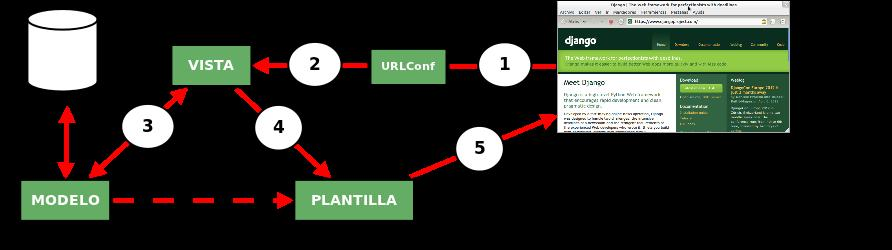
\includegraphics[scale=0.5]{imagenes/arquitectura_django.jpg}
   \caption{Componentes del computador}\label{graf:arquitectura-django}
\end{figure}

En la gráfica \ref{graf:arquitectura-django} \cite{Infante2012} se ve la relación entre los tres elementos fundamentales del framework: El modelo, las vistas y los templates.\\

\subsection*{El Modelo}

El modelo define los datos guardados en una BD mediante clases de Python. El modelom puede tener métodos también que operen sobre los datos del modelo.

\subsection*{La Vista}

Las vistas son funciones de Python e implementan las reglasde negocio entre el modelo de datos y la representación de cara al usuario. No tiene que ver con la forma de presentar los datos, de eso se encargan los templates.

\subsection*{El Template}

Los templates son páginas HTML con algunas etiquetas propias de Django. En un template puede haber css, javascript y cualquier elemento propio de una página web. Además de HTML Django también puede crear otro tipo de texto plano como XML, CSV.\\

En las plantillas Django implementa cierta lógica de tal modo que se pueda iterar sobre listas, definir cuando presentar o no una parte de la página. Es una lógica limitada de tal forma que las reglas de negocio sigan estando en las vistas.

\subsection{Mapeo de URLs}

En Django se mapean las urls de tal manera que forman un mapa de la aplicación, controlando la ejecución de las vistas. URLConf lee la url solicitada por el usuario, encuentra la vista apropiada y pasa las variables necesarias. URLConf funciona mediante expresiones regulares.\\

Es mediante URLConf que las urls en Django son agradables y se les puede aplicar patrones para su uso intuitivo por parte del usuario.\\


\section{Ejercicios}

\begin{enumerate}
\item Escriba una aplicación utilizando el Framework Django que consista en un modelo Persona y dos modelos: PersonaNatural y PersonaJuridica que hereden del anterior los atributos en común. Edite los atributos de cada modelo mediante la interfaz de administración de Django.

\item Escriba una aplicación "Hora" que consista en una vista que devuelva la hora cada vez que se refresque la pantalla.

\item Escriba una aplicación donde exista un modelo Mascota con un ForeignKey a un modelo Especie (dos los atributos sean los de las especies de mascotas) y a un modelo Propietario (con los atributos de una persona natural propietaria de una mascota). Escriba una vista donde se muestre una tabla de las Mascotas existentes con sus atributos y los nombres de sus dueños y especies..

\item Introduzca por lo menos diez mascotas en la aplicación anterior. Escriba un formulario de búsqueda donde se filtre el modelo por el nombre de la mascota.

\item Crear un formulario donde se se tenga un campo de texto. En este campo de texto ingresar alguna palabra y cuando se presione el botón de Enviar debe verse la palabra ingresada en la pantalla.

\item Crear un formulario que modifique el modelo Persona Natural del ejercicio 1.

\item Crear un formulario que busque en el modelo Mascota. El formulario debe tener un campo por cada campo del modelo Mascota y al presionarse Enviar se deben ver los resultados obtenidos.
\end{enumerate}



